\documentclass{article}
\usepackage[utf8]{inputenc}
\usepackage{graphicx}
\usepackage{subcaption}
\usepackage{placeins}

\title{Machine Learning\\Homework Assignment 1}
\author{Yuntong Wang\\UNI: yw2768}
\date{\today}

\begin{document}

\maketitle

\section{Problem 1}

\subsection{Part 1}

(a) Since the probability mass function for Bernoulli distribution is:
$$ p(x_i|\theta) = \pi^{x_i}(1-\pi)^{1-x_i} $$
Let $\Sigma$ denotes the sum of the sequence of $N$ observations. That is  $\Sigma = \displaystyle \sum_{i=1}^{N}x_i$. So the joint likelihood of the data $(x_1,...,x_N)$ is:
$$\prod_{i=1}^{N}p(x_i|\theta) = \pi^\Sigma(1-\pi)^{N-\Sigma}$$
(b) The maximum likelihood estimate $\hat{\pi}_{ML}$ for $\pi$ is:
$$\hat{\pi}_{ML}= \arg \max_{\pi}\pi^\Sigma(1-\pi)^{N-\Sigma}$$
Find $\pi$ that makes $\nabla_{\pi}\pi^\Sigma(1-\pi)^{N-\Sigma}=0$ :
$$\Sigma\pi^{\Sigma-1}(1-\pi)^{N-\Sigma} - \pi^{\Sigma}(1-\pi)^{N-\Sigma-1}(N-\Sigma) = 0$$
$$\Sigma\pi^{-1}-\Sigma-N+\Sigma = 0$$
$$\pi = \frac{\Sigma}{N}$$
So the result is:
$$\hat{\pi}_{ML} = \frac{1}{N}{\displaystyle \sum_{i=1}^{N}x_i}$$
(c) Since Bernoulli random variables takes value 1 as success with probability $\pi$ and value 0 as failure with probability $1-\pi$. So the expectation value for Bernoulli random variable is $1\cdot\pi+0\cdot(1-\pi) = \pi$. Therefore, in a sequence of $N$ observations, ${\displaystyle \sum_{i=1}^{N}x_i}$ is how many times we get a success, which is of probability $\pi$, out of $N$ observations. So this maximum likelihood estimate can be seen as the probability we can get a success whenever given a random variables from this particular observation set. So, intuitively, that's the estimate $\pi$ we can get from the data we already have.

\subsection{Part 2}

(a) Since the probability mass function for Poisson distribution is:
$$ p(x_i|\lambda) = \frac{\lambda^{x_i}e^{-\lambda}}{{x_i}!} $$
So the joint likelihood of the data $(x_1,...,x_N)$ is:
$$p(x_1,...,x_N|\lambda) = \prod_{i=1}^{N}\frac{\lambda^{x_i}e^{-\lambda}}{{x_i}!}$$
$$\hat{\lambda}_{ML} = \arg \max_{\lambda}\sum_{i=1}^{N}\ln(\frac{\lambda^{x_i}e^{-\lambda}}{{x_i}!})$$
Find $\lambda$ that makes $\displaystyle \sum_{i=1}^{N}\nabla_{\lambda}\ln(\frac{\lambda^{x_i}e^{-\lambda}}{{x_i}!})=0$ :
$$\displaystyle \sum_{i=1}^{N}\frac{1}{\lambda^{x_i}e^{-\lambda}}(x_i\lambda^{x_i-1}e^{-\lambda}-\lambda^{x_i}e^{-\lambda}) = 0$$
$$\displaystyle \sum_{i=1}^{N}(\frac{x_i}{\lambda}-1) = 0 $$
$$\frac{1}{\lambda}\displaystyle \sum_{i=1}^{N}x_i = N$$
So the result is:
$$\hat{\lambda}_{ML} = \frac{1}{N}\displaystyle \sum_{i=1}^{N}x_i$$
(c) Since the expectation value for Poisson-distribution random variable is $\lambda$. So it's reasonable and intuitively to guess $\lambda$ as the mean value of the whole data set.
\section{Problem 2}
(a) From Bayes Rule, the posterior distribution of $\lambda$ giving $(x_1,...,x_N)$:\\
$$ p(\lambda|x_1,...,x_N) = \frac{p(x_1,...,x_N|\lambda)p(\lambda|a,b)}{\int_0^1{p(x_1,...,x_N|\lambda)p(\lambda|a,b)}d\lambda } $$

$$ p(\lambda|x_1,...,x_N) \propto p(x_1,...,x_N|\lambda)p(\lambda|a,b) $$

$$  \propto \prod_{i=1}^{N}\frac{\lambda^{x_i}e^{-\lambda}}{{x_i}!}   \frac{b_a}{\Gamma(a)}\lambda^{a-1}e^{-b\lambda}$$

$$\propto \lambda^{\sum_{i=1}^{N}x_i+a-1}e^{-(N+b)\lambda}
$$

We recognize this as $p(\lambda|x_1,...,x_N) = Gam(\displaystyle \sum_{i=1}^{N}x_i+a, N+b )$\\
(b) Since from last problem, we derive that $\lambda ~ Gam(\lambda|\displaystyle \sum_{i=1}^{N}x_i+a, N+b )$. So the mean and variance of $\lambda$ are:\\
$$ mean [\lambda] = \frac{ \sum_{i=1}^{N}x_i+a}{N+b}$$
$$ variance[\lambda] = \frac{ \sum_{i=1}^{N}x_i+a}{(N+b)^2}$$
compared to the mean value for Part 2 of problem 1 that $\hat{\lambda}_{ML} = \frac{1}{N} \sum_{i=1}^{N}x_i$, which only maximizes the likelihood. But in this problem, $ mean [\lambda] $ not only maximizes the likelihood, but also takes the prior distribution of $\lambda$ into account. It uses Bayes rule to seek out the most probable value of $\lambda$ under prior distribution of $\lambda$.

\section{Problem 3}
\subsection{Part 1}

(a) The numbers obatined for the vector $\hat{w}_{ML}$ was printed in MATLAB:\\\\
Parameters $\hat{w}_{ML}$ obtained from linear regression using least square: 
\FloatBarrier
\begin{table}[h!]
\centering
\begin{tabular}{|c|c|}
 \hline
Label       & parameter value\\
 \hline
intercept term      & 23.4164\\
 \hline
number of cylinders & -0.4922\\
 \hline
displacement        & 0.7757\\
 \hline
horsepower          & 0.1613\\
 \hline
weight              & -5.9491\\
 \hline
acceleration        & 0.3354\\
 \hline
model year          & 2.8201\\
\hline
\end{tabular}
\end{table}
\FloatBarrier
The results shows that the miles per gallon a car will get is affected by different factors in different degrees.
The sign of each value in $\hat{w}_{ML}$ indicates whether the attribute in this dimension affects miles per gallon positively or negatively. For example, number of cylinders and weight are with negative sign, which means that miles per gallon will decrease with these two values increase. On the other hand, miles per gallon will increase with parameters displacement, horsepower, acceleration and model year increase.\\\\
(b) The mean and standard deviation of the MAE for these 1000 tests are showed below:\\\\
Statistics on the MAE for these 1000 tests: \\
Mean              : 2.67\\
Standard deviation: 0.48\\
\subsection{Part 2}
(a)The mean and standard deviation of the RMSE as a function of $p$ are printed below:
\FloatBarrier
\begin{table}[h!]
\centering
\begin{tabular}{|c|c|c|}
 \hline
p  &   $Mean_{RMSE}$   &   $Std_{RMSE}$\\
\hline
1& 3.4079&    0.6510\\
\hline
2& 2.7284&    0.6179\\
\hline
3& 2.6307&    0.6209\\
\hline
4& 2.6749&    0.5898\\
\hline
\end{tabular}
\end{table}
\FloatBarrier
These data shows that 3 for the value of $p$ is the best. Because this pair of numbers have the least mean value and standard deviation of RMSE. So it minimizes the root mean squared error, which makes it best.\\\\
(b)The histogram of error: $y^{test} - y^{pred}$  for each p are showed below:\\
\FloatBarrier
\begin{figure}[h]
\begin{subfigure}{0.5\textwidth}
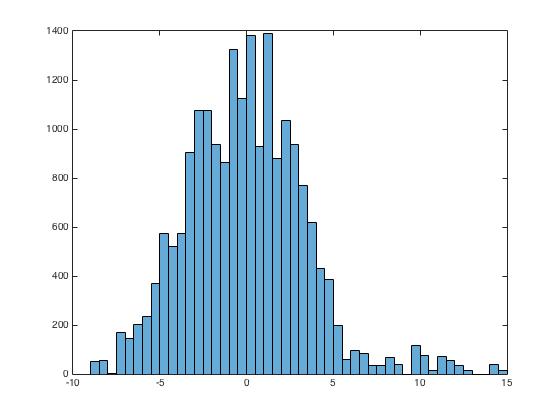
\includegraphics[width=0.9\linewidth, height=5cm]{hist1} 
\caption{p = 1}
\label{fig:subim1}
\end{subfigure}
\begin{subfigure}{0.5\textwidth}
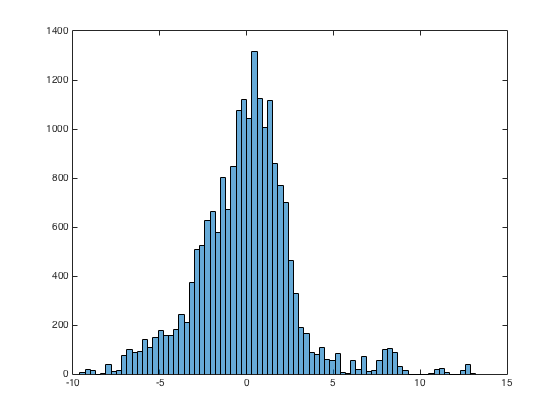
\includegraphics[width=0.9\linewidth, height=5cm]{hist2}
\caption{p = 2}
\label{fig:subim2}
\end{subfigure}
 \begin{subfigure}{0.5\textwidth}
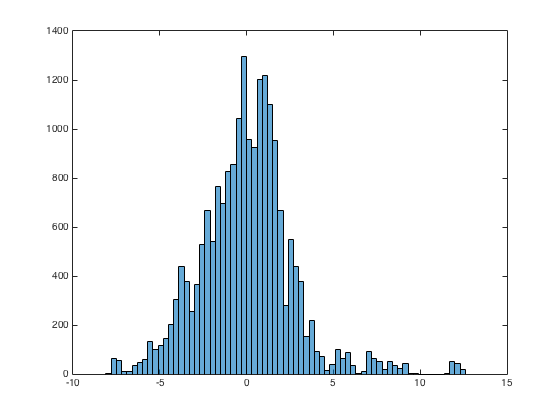
\includegraphics[width=0.9\linewidth, height=5cm]{hist3}
\caption{p = 3}
\label{fig:subim3}
\end{subfigure}
\begin{subfigure}{0.5\textwidth}
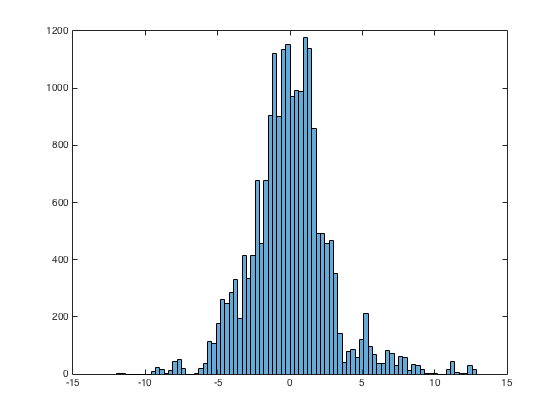
\includegraphics[width=0.9\linewidth, height=5cm]{hist4}
\caption{p = 4}
\label{fig:subim4}
\end{subfigure}
\caption{Histogram for p = 1,2,3,4}
\label{fig:image2}
\end{figure}
\FloatBarrier\\\\
(c) Since we need to use maximum likelihood to fit a univariate Gaussian model. So from the derivation of multivariate Gaussian of class, we can calculate the maximum likelihood values for the mean and variance like this:\\
$$\hat{\mu}_{ML} = \frac{1}{N}\displaystyle \sum_{i=1}^{N}x_i$$
$$\hat{\Sigma}_{ML} = \frac{1}{N}\displaystyle \sum_{i=1}^{N}(x_i - \hat{\mu}_{ML})^2$$
where $x_i$ is a sample error data $y^{test} - y^{pred}$ from previous questions. $N = 20,000$.\\
For each $p$, the parameters of univariate Gaussian to the 20,000 errors from Part 2(b) are showed below:
\FloatBarrier
\begin{table}[h!]
\centering
\begin{tabular}{|c|c|c|}
\hline
$p$&  $\hat{\mu}_{ML}$   &   $\hat{\Sigma}_{ML}$\\
\hline
1&0.0397&   3.4807\\
\hline
2&0.0164&   2.8194\\
\hline
3&0.0143&   2.7268\\
\hline
4&0.0027&   2.7494\\
\hline
\end{tabular}
\end{table}
\FloatBarrier
Log likelihood of these empirical errors using the maximum likelihood value for the mean and variance are showed below as a function of $p$:
\FloatBarrier
\begin{table}[h!]
\centering
\begin{tabular}{|c|c|}
\hline
p&  log likelihood\\
\hline
1&-53323.1746\\
\hline
2&-49109.1569\\
\hline
3&-48441.6789\\
\hline
4&-48606.5221\\
\hline
\end{tabular}
\end{table}
\FloatBarrier
This agrees with the conclusion in Part 2(a). Because in this approach, p for the value $p$ is also the best since it maximizes the log likelihood. So we can construct out prediction function with $p = 3$. That is:
$$y^{pred} = w_{0} + \sum_{p=1}^{3}\sum_{j=1}^{6}x_{j}^{p}w_{p,j}$$

\end{document}
